
% Comandos de dados - titulo do documento
\newcommand{\titulo}[1]{\title{#1}}
\newcommand{\imprimirtitulo}{\thetitle}

% Comandos de dados - autor (use \and para múltiplos autores)
\newcommand{\autor}[1]{\author{#1}}
\newcommand{\imprimirautor}{\theauthor}

% Comandos de dados - data
\let\olddate\date
\renewcommand{\date}[1]{\AtBeginDocument{\olddate{#1}}}
\newcommand{\data}[1]{\date{#1}}
\newcommand{\imprimirdata}{
  \center
  \the\year
}

% Comandos de dados - instituição
\providecommand{\imprimirinstituicao}{}
\newcommand{\instituicao}[1]{\renewcommand{\imprimirinstituicao}{#1}}

% Comandos de dados - local
\providecommand{\imprimirlocal}{}
\newcommand{\local}[1]{\renewcommand{\imprimirlocal}{#1}}

% Comandos de dados - preambulo
\providecommand{\imprimirpreambulo}{}
\newcommand{\preambulo}[1]{\renewcommand{\imprimirpreambulo}{#1}}

% Comandos de dados - orientador
\providecommand{\imprimirorientadorRotulo}{}
\providecommand{\imprimirorientador}{}
\newcommand{\orientador}[2][\orientadorname]%
  {\renewcommand{\imprimirorientadorRotulo}{#1}%
   \renewcommand{\imprimirorientador}{#2}}

% Comandos de dados - coorientador
\providecommand{\imprimircoorientadorRotulo}{}
\providecommand{\imprimircoorientador}{}
\newcommand{\coorientador}[2][\coorientadorname]%
  {\renewcommand{\imprimircoorientadorRotulo}{#1}%
   \renewcommand{\imprimircoorientador}{#2}}

% Comandos de dados - tipo de trabalho
\providecommand{\imprimirtipotrabalho}{}
\newcommand{\tipotrabalho}[1]{\renewcommand{\imprimirtipotrabalho}{#1}}


\newcommand{\imprimircapa}{%
  \begin{capa}%
    \center
    \imprimirinstituicao
    \vfill
    \large\imprimirautor

    \vfill
    \begin{center}
      \MakeUppercase{\imprimirtitulo}
    \end{center}
    \vfill

    \large\imprimirlocal

    \large\imprimirdata

    \vspace*{1cm}
  \end{capa}
}

\newenvironment{capa}{\begin{titlingpage}}{\end{titlingpage}\cleardoublepage}

% ---
% Folha de rosto
%   usar \imprimirfolhaderosto* caso deseje imprimir algo no verso da
%   página no caso de estar no modo twoside. Util para imprimir a Ficha
%   Bibliográfica. Porem, se estiver no modo oneside, a versao sem estrela é idêntica.
\newenvironment{folhaderosto}[1][\folhaderostoname]{\clearpage}{\cleardoublepage}
\newenvironment{folhaderosto*}[1][\folhaderostoname]{\clearpage}{\newpage}%

% ---
% Conteudo padrao da Folha de Rosto
\makeatletter
\newcommand{\folhaderostocontent}{
  \begin{center}
    \imprimirinstituicao\vspace*{\fill}

    \large\imprimirautor

    \vspace*{\fill}\vspace*{\fill}
    \begin{center}
      \MakeUppercase{\imprimirtitulo}
    \end{center}
    \vspace*{\fill}

    \hspace{.45\textwidth}
    \begin{minipage}{.5\textwidth}
    	\singlespacing
       \imprimirpreambulo
     \end{minipage}
     \vspace*{\fill}

    \begin{flushright}
        \large\imprimirorientadorRotulo
        \imprimirorientador\par
        \vspace*{\fill}  
    \end{flushright}


    \large\imprimirlocal
    \par
    \large\imprimirdata
    \vspace*{1cm}

  \end{center}
}
\makeatother

\newcommand{\imprimirfolhaderostostar}[1]{%
  \begin{folhaderosto*}{#1}
     \folhaderostocontent
  \end{folhaderosto*}}

\newcommand{\imprimirfolhaderostonostar}[1]{%
  \begin{folhaderosto}{#1}
     \folhaderostocontent
  \end{folhaderosto}}

\makeatletter
\newcommand{\imprimirfolhaderosto}[1][\folhaderostoname]{%
   \@ifstar
     \imprimirfolhaderostostar
     \imprimirfolhaderostonostar
}
\makeatother


\documentclass[12pt]{article}
\usepackage{titling}
\usepackage{sbc-template}
\usepackage{graphicx}
\usepackage{float}
\PassOptionsToPackage{hyphens}{url}%\usepackage{hyperref}
\usepackage{url}
\usepackage{minted}

\usepackage[brazil]{babel}
\usepackage[utf8]{inputenc}

\usepackage{multicol}
\usepackage{multirow}
\usepackage{setspace,lipsum}

\sloppy



\date{\today}

\title{
    Cobertura vacinal de HPV, dengue e meningite bacteriana em adolescentes em 2024
}

\local{Porto Alegre}

\author{Tiago Sturmer-Daitx\inst{1}}

\preambulo{Artigo apresentado como requisito parcial para obtenção do título de Especialista em \textbf{Engenharia de Software}, pelo Curso de Especialização em \textbf{Engenharia de Software} da Universidade do Vale do Rio dos Sinos – UNISINOS}

\address{Universidade do Vale do Rio dos Sinos (UNISINOS)\\
  Av. Unisinos, 950, Bairro Cristo Rei, São Leopoldo, RS -- Brasil
}

%\orientador{Orientador(a): Prof(a). Ms. \textbf{}}

\instituicao{
    UNIVERSIDADE DO VALE DO RIO DOS SINOS - UNISINOS

    UNIDADE ACADÊMICA DE EDUCAÇÃO CONTINUADA

    ESPECIALIZAÇÃO EM ENGENHARIA DE SOFTWARE
}

\begin{document}

\imprimircapa
\imprimirfolhaderosto


\maketitle

\begin{abstract}
This study investigates the vaccination coverage of adolescents under SUS's Basic Vaccination Calendar, highlighting the recent availability of dose administration data. Despite the critical importance of adolescent vaccination for public health,  the analysis reveals significant disparities in vaccination coverage. Comprehensive investigation on this demographic remain scarce, emphasizing the need for more studies. The findings underscore the potential benefits of enhanced data automation with opensource tools in exploring open vaccination data, ultimately contributing to improved health outcomes for adolescents.
\end{abstract}

\begin{resumo}
Este estudo investiga a cobertura vacinal de adolescentes sob o Calendário Básico de Vacinação do Sistema Único de Saúde (SUS), destacando a recente disponibilidade de dados sobre a aplicação de doses. Apesar da importância crítica da vacinação de adolescentes para a saúde pública, a análise revela disparidades significativas na cobertura vacinal. Investigações abrangentes sobre essa demografia ainda são escassos, enfatizando a necessidade de mais estudos. Os resultados ressaltam os benefícios potenciais do uso de ferramentas livres para automação da exploração de dados abertos de vacinação, contribuindo, em última análise, para melhores resultados de saúde para os adolescentes.
\end{resumo}


\section{Introdução} \label{introducao}

A imunização se destaca como uma das intervenções mais eficazes no controle de várias doenças e faz parte da estratégia da Agenda de Imunização 2030 da Organização Mundial da Saúde \cite{who_ia2030_2021}. No Brasil, o Programa Nacional de Imunizações (PNI), criado em 1973, é uma iniciativa vital de saúde pública que visa garantir a vacinação da população contra doenças imunopreveníveis, estabelece o calendário vacinal e distribui vacinas gratuitamente em todo o país. Coordenado pelo Ministério da Saúde, o PNI realiza campanhas de vacinação com vacinas essenciais como BCG, hepatite B e tríplice viral (sarampo, caxumba e rubéola). Com um sistema eficiente de distribuição, o programa alcançou coberturas vacinais acima de 90\% para diversas vacinas, essencial para o controle de doenças como o sarampo e poliomielite \cite{ministerio_da_saude_programa_2024}.

Apesar do sucesso do PNI, a taxa de vacinação teve um grande período de quedas a partir de 2016 e só voltou a subir em 2022, porém sem atingir os patamares de 2015 \cite{domingues_vacina_2019} \cite{fontanetto_reconquista_2024}, influenciada pelo fenômeno da "hesitação vacinal" e por dificuldades encontradas no processo de vacinação. A hesitação vacinal é a relutância em aceitar vacinas, mesmo quando disponíveis, e é influenciada por fatores como desinformação, preocupações com segurança e crenças culturais. Esse fenômeno pode comprometer campanhas de imunização e levar ao ressurgimento de doenças controladas. Para combatê-lo, é essencial promover educação sobre a importância das vacinas e incentivar um diálogo aberto entre profissionais de saúde e a comunidade. As dificuldades de vacinação estão relacionadas à falta de imunizante, salas de vacinação fechadas, distância do posto, falta de meio de transporte, horário de funcionamento inadequado, dentre outros \cite{barata_inquerito_2023}.

A cobertura vacinal é o indicador mais relevante para a avaliação e o monitoramento da vacinação em grande escala. Ela demonstra se a população-alvo recebeu as vacinas necessárias e, ao ser acompanhada, revela a eficácia do programa de imunização. Esse indicador também desempenha um papel crucial na análise do sistema de saúde, da atenção primária à saúde (APS) e dos serviços de vacinação em um país específico \cite{pamplona_imunizacao_2020}. Acompanhar a cobertura vacinal da população é fundamental para garantir a eficácia das campanhas de imunização e a proteção coletiva contra doenças \cite{shattock_contribution:2024}. A monitorização permite identificar áreas com baixa adesão às vacinas, possibilitando intervenções mais direcionadas e eficazes. Isso é crucial para evitar surtos de doenças que podem ser prevenidas por vacinas, além de assegurar que a população, especialmente os grupos mais vulneráveis, esteja adequadamente protegida.

As vacinas mais importantes se concentram desde o nascimento ao primeiro ano da criança, assim como gestantes, constando no Calendário Básico de Vacinação do Sistema Único de Saúde (SUS) e, consequentemente, são as que possuem maior acompanhamento nos programas de governo \cite{silva_protegendo_2024}. O painel de monitoramento do Departamento de Monitoramento, Avaliação e Disseminação de Informações Estratégicas em Saúde (DEMAS) da Secretaria de Informação e Saúde Digital (SEIDIGI) disponibiliza os índices de cobertura vacinal para 19 vacinas por região de residência, unidade da federação (UF), macroregião, região de saúde, região de fronteira, cidade gêmea e município para crianças até um ano e gestantes \cite{demas_cobertura_2024}.

Dentre as vacinas de rotina para crianças e adolescentes, de 9 a 14 anos, cobertas pelo Calendário Básico do SUS estão a vacina HPV quadrivalente, a Meningocócica ACWY e a vacina contra a dengue. A vacina HPV quadrivalente (HPV4) é essencial para prevenir infecções por quatro tipos do vírus do papiloma humano (HPV), que estão associados ao câncer de colo de útero e outras neoplasias \cite{adames_hpv_2023}. O SUS oferece essa vacina para meninas e meninos de 9 a 14 anos, que são mais suscetíveis à infecção \cite{informe_ms_hpv4:2018} \cite{ms_risco_hpv_cancer:2024}.

A vacina Meningocócica ACWY (MenACWY) protege contra quatro sorogrupos da bactéria Neisseria meningitidis, responsável por meningites e septicemias graves. A doença mata 1 em cada 10 pessoas infectadas, especialmente crianças, e deixa 1 em cada 5 com incapacidades de longa duração, como convulsões, perda de audição e visão e deficiência cognitiva. É recomendada para crianças e adolescentes de 11 a 14 anos. Essa faixa etária é especialmente importante, pois os casos tendem a ser assintomáticos, que leva a um maior risco de transmissão e complicações associadas \cite{who_defeating_2021} \cite{ms_risco_meningite:2022}.

Por fim, a vacina contra a dengue é crucial em regiões onde a doença é endêmica. O Calendário Básico prevê a vacinação em crianças e adolescentes, de 10 a 14 anos, e busca reduzir não apenas os casos da doença, mas também as hospitalizações e complicações graves associadas à dengue \cite{ms_risco_dengue:2024}. As crianças e  adolescentes que não se vacinam dentro do calendário perdem a oportunidade de receber essas vacinas devido à idade.

Apesar da importância dessas vacinas, em consulta por buscadores na internet, não foi identificado um monitoramento abrangente da cobertura vacinal de crianças e  adolescentes, apenas algumas notas informativas de ministérios regionais sem detalhes sobre a metodologia e sem referências. Em consultas por artigos no CAPES foram encontrados estudos anteriores cobrindo o acompanhamento da vacina HPV4 até 2019 na região Sul \cite{adames_hpv_2023}, outro até 2017 de todo Brasil estratificado em microrregiões \cite{moura_cobertura_2021} e um estudo do estado vacinal de escolares matriculados do 4º ao 9º ano em escolas municipais de Palmas/TO cobrindo as vacinas HPV4 e MenACWY \cite{sousa_alencar_cantuaria_estado_2024}. Não foram encontrados estudos de cobertura para a vacina contra Dengue, que começou a ser aplicada no início de 2024.

Diante desse cenário, o presente estudo busca contribuir para o entendimento da cobertura vacinal das três vacinas selecionadas nas cinco regiões do Brasil. Utilizando dados disponíveis publicamente para o ano de 2024, este trabalho visa não apenas preencher as lacunas existentes na literatura sobre vacinação de crianças e adolescentes no Brasil com as vacinas contra dengue, HPV4 e MenACWY, mas também oferecer uma base sólida para intervenções futuras e políticas públicas mais eficazes. Somado a isso, esse estudo visa explorar ferramentas simples de leitura, armazenamento e processamento de dados massivos para automatizar os resultados conforme mais dados são disponibilizados pelos portais.

\section{Fundamentação Teórica} \label{sec:fundamentacao teorica}
Na literatura, a cobertura vacinal pode ser definida de diversas formas \cite{pamplona_imunizacao_2020} e é um indicador crucial para avaliar o desempenho dos programas públicos de vacinação além de ajudar na identificação de áreas vulneráveis ao retorno de doenças evitáveis por imunização e na verificação do cumprimento das metas estabelecidas pelo PNI \cite{observatorio_das_vacinas_mapa_2020}.
Neste estudo, utilizamos a seguinte definição: cobertura vacinal reflete a fração da população-alvo que foi vacinada em relação a uma vacina específica em um determinado tempo e espaço, dada pela seguinte fórmula

\begin{figure}[ht]
    \centering
    \textbf{Cálculo da cobertura vacinal}
    \[
        \parbox[ht]{3.3cm}{\raggedleft Cobertura vacinal da população alvo} =
        \sum_{ti}^{tf}
        {\left(\frac{100 * \mbox{doses aplicadas na população alvo}}{\mbox{quantidade de pessoas da população alvo}}\right)}
    \]
\end{figure}

onde \emph{população alvo} é representada pela fração de adolescentes dentro da região estratificada que cumprem os requisitos de idade da vacina, $ti$ é a data inicial e $tf$ é a data final. Neste estudo o período $(tf-ti)$ foi escolhido de forma que cubra 12 meses e representa a cobertura vacinal na data $tf$. Exemplo: a cobertura vacinal de Junho de 2024, para uma dada vacina, considera a soma de todas as doses aplicadas na população alvo, no período de 01/07/2023 até 30/06/2024, dividida pelo tamanho da população alvo no período.

É importante observar que uma das definições de cobertura vacinal, a chamada cobertura vacinal completa, somente leva em consideração a aplicação da última dose ou da dose única. Neste estudo a cobertura completa é dada pela soma da dose única com a segunda dose (ou dose de reforço).

A cobertura vacinal foi categorizada levando em consideração as metas
recomendadas pelo PNI e Organização Mundial da Saúde (OMS). A meta de cobertura
vacinal adequada são valores iguais ou maiores de 80\% para a vacina MenACWY e 90\% para as vacinas HPV4 e dengue, conforme a tabela \ref{tab:classificacao de cobertura vacinal}.

\begin{table}[ht]
    \centering
    \caption{Classificação de cobertura vacinal}
    \label{tab:classificacao de cobertura vacinal}
    \begin{tabular}{lc}
        \hline
        \rule[-1ex]{0pt}{2.5ex} \textbf{Valores} & \textbf{Classificação da cobertura vacinal} \\
        \hline
        \rule[-1ex]{0pt}{2.5ex} 0 a 49,9\% & Muito baixa \\
        \hline
        \rule[-1ex]{0pt}{2.5ex} 50 a menor que a meta (80/90\%) & Baixa \\
        \hline
        \rule[-1ex]{0pt}{2.5ex} Meta (80/90\%) a 120\% & Adequada \\
        \hline
        \rule[-1ex]{0pt}{2.5ex} Maior que 120\% & Elevada \\
        \hline
    \end{tabular}
\end{table}

\section{Metodologia} \label{sec:metodologia}
Trata-se de um estudo exploratório, longitudinal e com abordagem quantitativa, realizado através do levantamento de dados públicos acerca da aplicação de doses de vacinas no ano de 2024, de janeiro a agosto, a partir do portal de dados abertos do DataSUS. Os dados de população foram obtidos pelo Sistema IBGE de Recuperação Automática (SIDRA), do censo de 2022.

\subsection{Dados}
O Sistema de Informa PNI (SI-PNI) registra as aplicações de doses tanto pelo programa de rotina quanto pelas campanhas de vacinação. Os dados são agregados na Rede Nacional de Dados em Saúde (RNDS) e disponibilizados pelos portais de dados abertos do Departamento de Informação e Informática do SUS (DataSUS) e do Governo Federal. Estavam disponíveis apenas no perído compreendido entre 1 de janeiro e 8 de agosto de 2024. Os dados de aplicação de doses estão no formato CSV, compactados em um arquivo ZIP, compreendendo todo um mês. Não existe um sistema para filtrar os dados previamente e todos os dados foram importados para um banco de dados SQLite local. Os dados foram processados, removendo registros com valores inválidos: país estrangeiro, município ou UF inválido e idade vazia.

Os dados para a vacina contra dengue passam a ser significantes apenas a partir da introdução da mesma no Calendário Básico do SUS, em fevereiro de 2024.

Posteriormente foram criadas consultas SQL, salvas como \emph{views}, para agregar a aplicação de doses por: região, UF, tipo de vacina e faixas etárias.

O SIDRA permite seleção prévia por região, UF, idade e possibilita a coleta dos dados em diversos formatos. Foi escolhido o formato CSV pela facilidade na importação ao banco de dados.

Todos os dados do censo são de 2022 e não incluem datas de nascimento, apenas a idade. Para o cálculo das vacinas a idade do censo foi ajustada seguindo a fórmula $i_a = (i_c + a_v - 2022)$, onde $i_c$ é a idade registrada no censo, $a_v$ é o ano onde ocorreu a vacinacão e $i_a$ é a idade ajustada. Exemplo: a população com idade de 10 anos no censo tinha 12 anos para vacinas aplicadas em 2024 ($10 + (2024 - 2022) = 12$).

Os dados agregados de doses e do censo foram extraídos por consultas SQL em formato de \emph{views} e importados em um \emph{notebook} Python, onde foram pós-processados com a ferramenta \emph{pandas} para a criação de gráficos.

\subsection{Percentual das doses aplicadas}
O percentual de doses aplicadas dentro da população alvo, calculada para cada vacina, estratificada por região, mês e ano, nas faixas etárias adequadas a cada uma. A agregação temporal dos dados foi feita por mês e ano, enquanto a espacial foi por região.

\subsubsection{Dengue}

\begin{figure}[H]
    \centering
    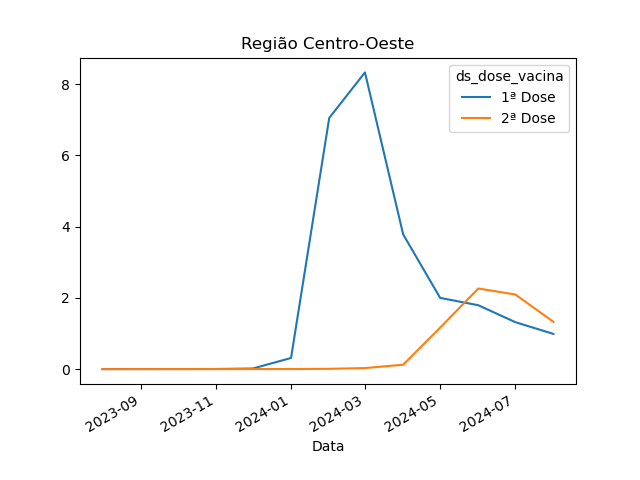
\includegraphics[width=0.85\linewidth]{imagens/Dengue-Centro-Oeste-Aplicacoes-mes}
    \caption{Dengue - Aplicações por mês - Centro-Oeste}
    \label{fig:dengue-centro-oeste-aplicacoes}
\end{figure}
\begin{figure}[H]
    \centering
    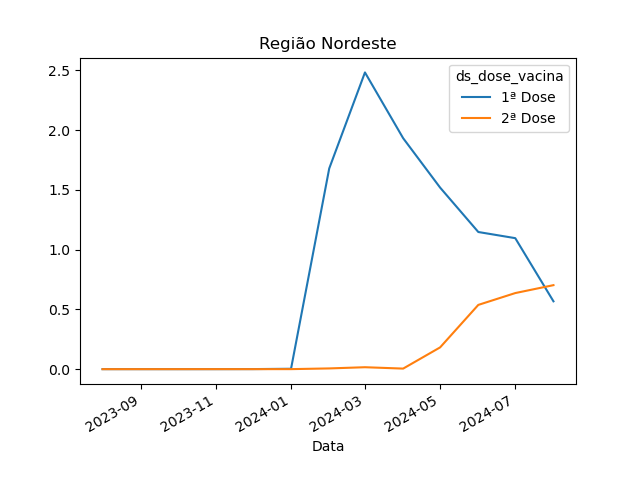
\includegraphics[width=0.85\linewidth]{imagens/Dengue-Nordeste-Aplicacoes-mes}
    \caption{Dengue - Aplicações por mês - Nordeste}
    \label{fig:dengue-nordeste-aplicacoes-mes}
\end{figure}
\begin{figure}[H]
    \centering
    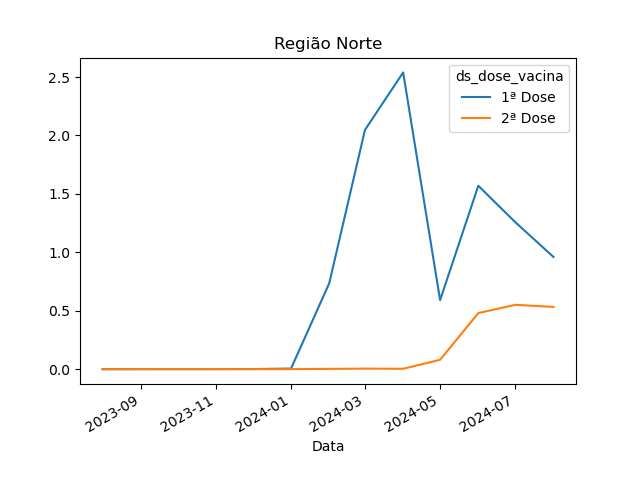
\includegraphics[width=0.85\linewidth]{imagens/Dengue-Norte-Aplicacoes-mes}
    \caption{Dengue - Aplicações por mês - Norte}
    \label{fig:dengue-norte-aplicacoes-mes}
\end{figure}
\begin{figure}[H]
    \centering
    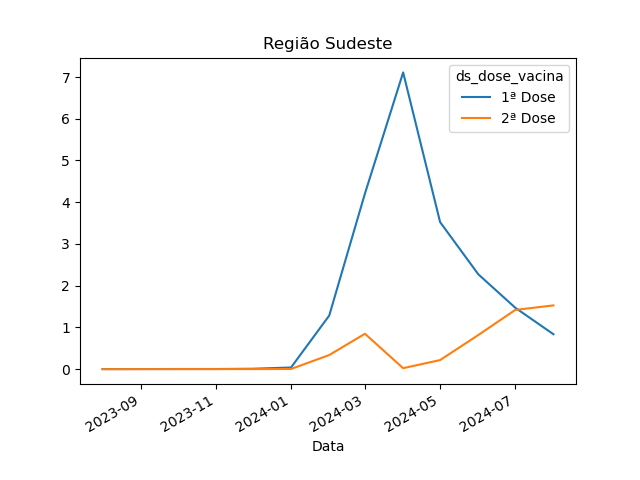
\includegraphics[width=0.85\linewidth]{imagens/Dengue-Sudeste-Aplicacoes-mes}
    \caption{Dengue - Aplicações por mês - Sudeste}
    \label{fig:dengue-sudeste-aplicacoes-mes}
\end{figure}
\begin{figure}[H]
    \centering
    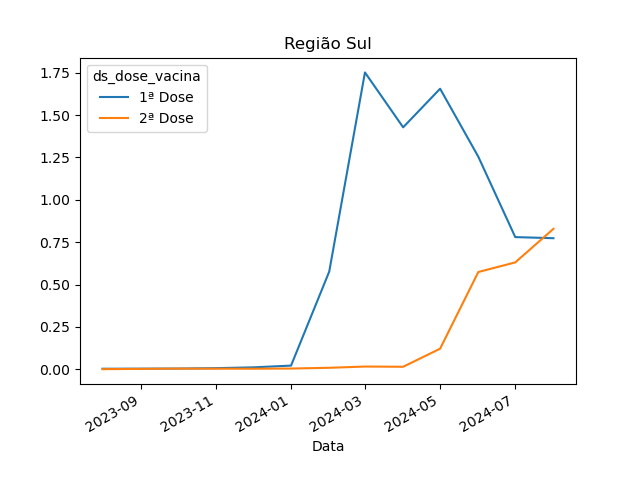
\includegraphics[width=0.85\linewidth]{imagens/Dengue-Sul-Aplicacoes-mes}
    \caption{Dengue - Aplicações por mês - Sul}
    \label{fig:dengue-sul-aplicacoes-mes}
\end{figure}

\subsubsection{HPV4}

\begin{figure}[H]
    \centering
    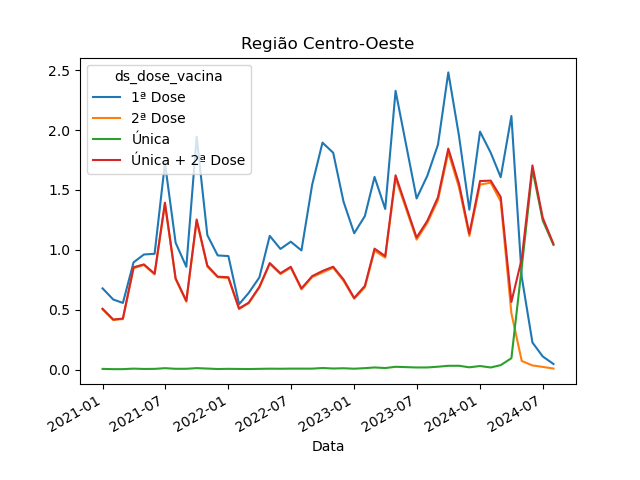
\includegraphics[width=0.85\linewidth]{imagens/HPV4-Centro-Oeste-Aplicacoes-mes}
    \caption{HPV4 - Aplicações por mês - Centro-Oeste}
    \label{fig:HPV4-centro-oeste-aplicacoes}
\end{figure}
\begin{figure}[H]
    \centering
    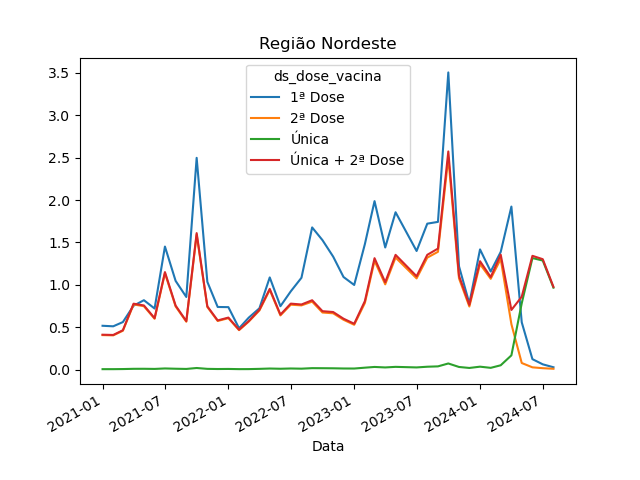
\includegraphics[width=0.85\linewidth]{imagens/HPV4-Nordeste-Aplicacoes-mes}
    \caption{HPV4 - Aplicações por mês - Nordeste}
    \label{fig:HPV4-nordeste-aplicacoes-mes}
\end{figure}
\begin{figure}[H]
    \centering
    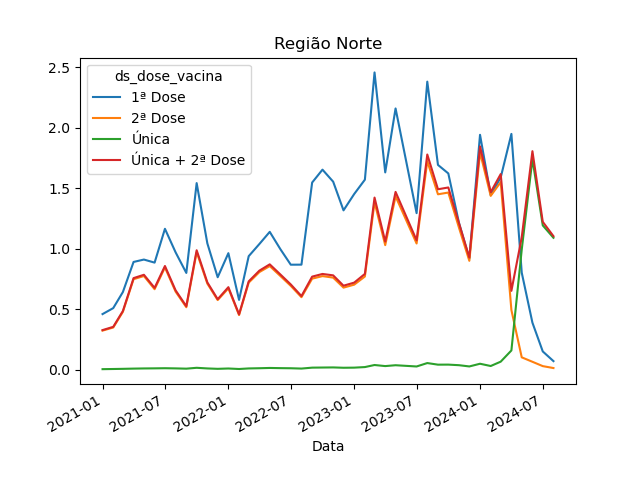
\includegraphics[width=0.85\linewidth]{imagens/HPV4-Norte-Aplicacoes-mes}
    \caption{HPV4 - Aplicações por mês - Norte}
    \label{fig:HPV4-norte-aplicacoes-mes}
\end{figure}
\begin{figure}[H]
    \centering
    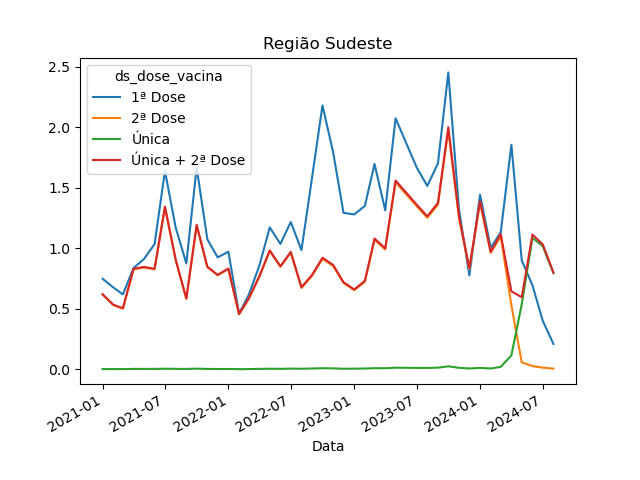
\includegraphics[width=0.85\linewidth]{imagens/HPV4-Sudeste-Aplicacoes-mes}
    \caption{HPV4 - Aplicações por mês - Sudeste}
    \label{fig:HPV4-sudeste-aplicacoes-mes}
\end{figure}
\begin{figure}[H]
    \centering
    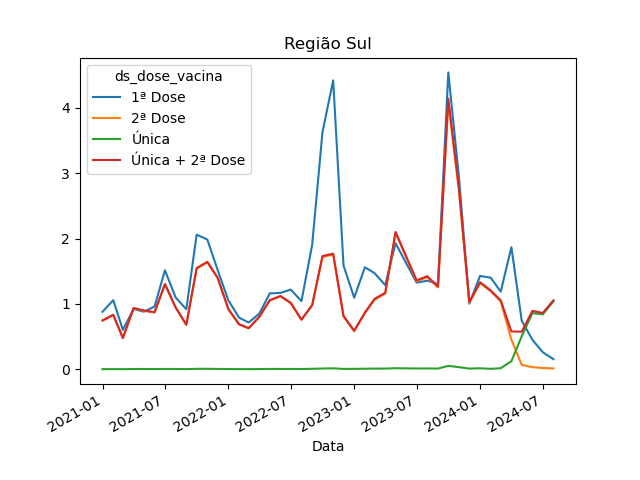
\includegraphics[width=0.85\linewidth]{imagens/HPV4-Sul-Aplicacoes-mes}
    \caption{HPV4 - Aplicações por mês - Sol}
    \label{fig:HPV4-sul-aplicacoes-mes}
\end{figure}

\subsubsection{MenACWY}
\begin{figure}[H]
    \centering
    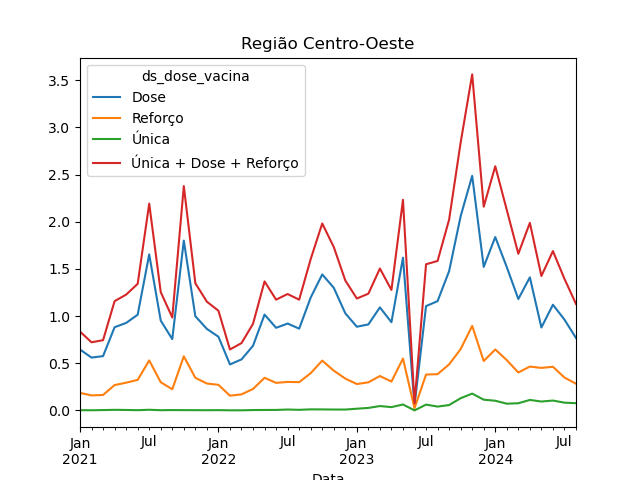
\includegraphics[width=0.85\linewidth]{imagens/MenACWY-Centro-Oeste-Aplicacoes-mes}
    \caption{MenACWY - Aplicações por mês - Centro-Oeste}
    \label{fig:MenACWY-centro-oeste-aplicacoes}
\end{figure}
\begin{figure}[H]
    \centering
    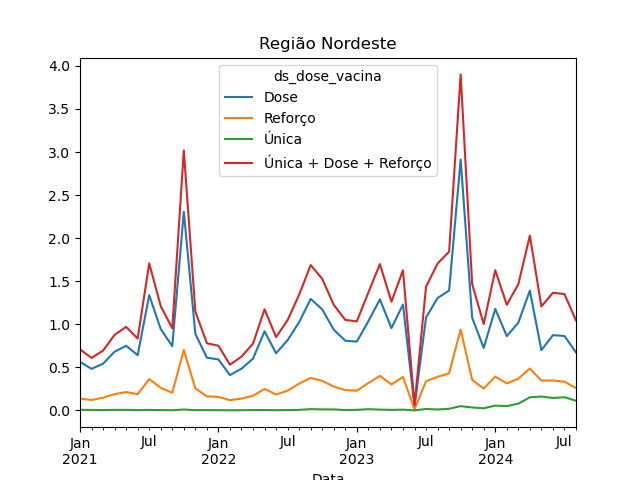
\includegraphics[width=0.85\linewidth]{imagens/MenACWY-Nordeste-Aplicacoes-mes}
    \caption{MenACWY - Aplicações por mês - Nordeste}
    \label{fig:MenACWY-nordeste-aplicacoes-mes}
\end{figure}
\begin{figure}[H]
    \centering
    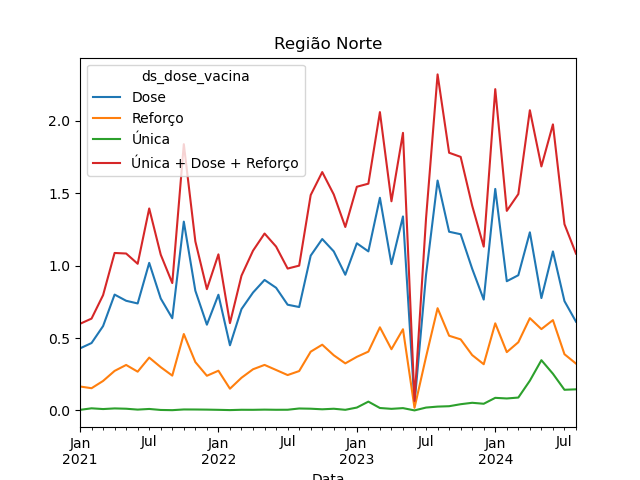
\includegraphics[width=0.85\linewidth]{imagens/MenACWY-Norte-Aplicacoes-mes}
    \caption{MenACWY - Aplicações por mês - Norte}
    \label{fig:MenACWY-norte-aplicacoes-mes}
\end{figure}
\begin{figure}[H]
    \centering
    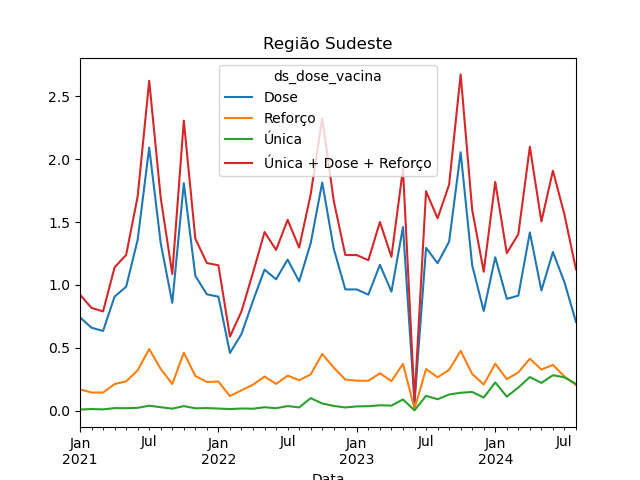
\includegraphics[width=0.85\linewidth]{imagens/MenACWY-Sudeste-Aplicacoes-mes}
    \caption{MenACWY - Aplicações por mês - Sudeste}
    \label{fig:MenACWY-sudeste-aplicacoes-mes}
\end{figure}
\begin{figure}[H]
    \centering
    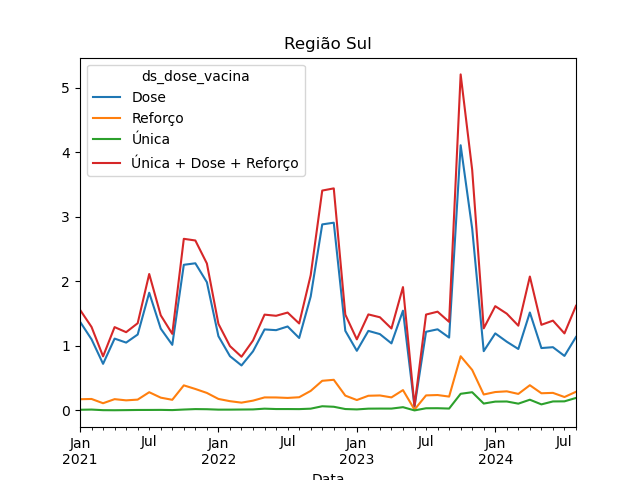
\includegraphics[width=0.85\linewidth]{imagens/MenACWY-Sul-Aplicacoes-mes}
    \caption{MenACWY - Aplicações por mês - Sol}
    \label{fig:MenACWY-sul-aplicacoes-mes}
\end{figure}


\subsection{Cobertura vacinal}
A cobertura vacinal calculada para cada vacina, estratificada por região, mês e ano, nas faixas etárias adequadas a cada uma.

\subsubsection{Dengue}
\begin{figure}[H]
    \centering
    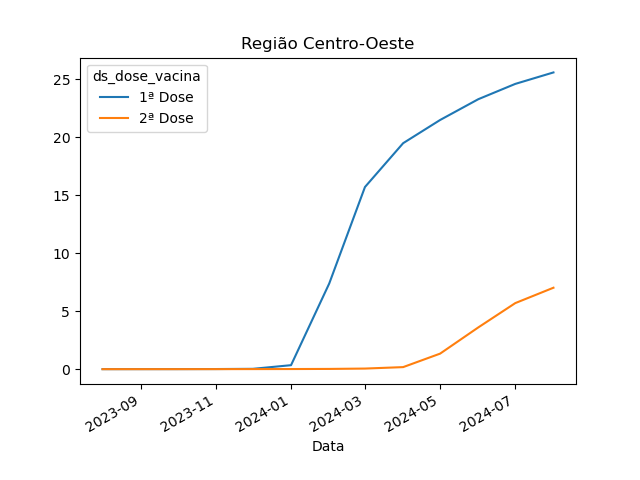
\includegraphics[width=0.85\linewidth]{imagens/Dengue-Centro-Oeste-Cumulativo-mes}
    \caption{Dengue - Cumulativo (últimos 12 meses) por mês - Centro-Oeste}
    \label{fig:dengue-centro-oeste-cumulativo}
\end{figure}
\begin{figure}[H]
    \centering
    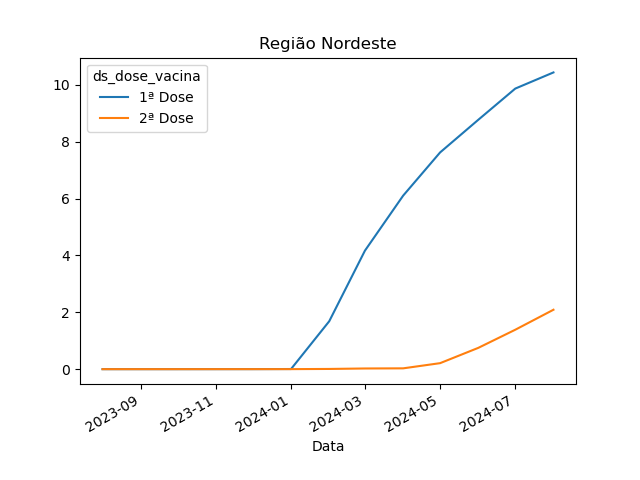
\includegraphics[width=0.85\linewidth]{imagens/Dengue-Nordeste-Cumulativo-mes}
    \caption{Dengue - Cumulativo (últimos 12 meses) por mês - Nordeste}
    \label{fig:dengue-nordeste-cumulativo-mes}
\end{figure}
\begin{figure}[H]
    \centering
    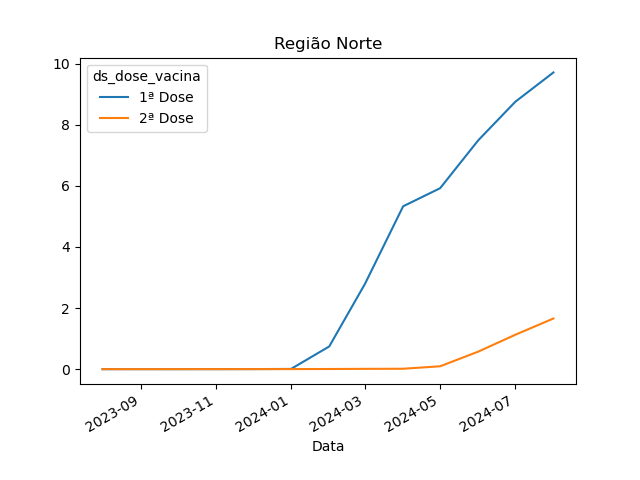
\includegraphics[width=0.85\linewidth]{imagens/Dengue-Norte-Cumulativo-mes}
    \caption{Dengue - Cumulativo (últimos 12 meses) por mês - Norte}
    \label{fig:dengue-norte-cumulativo-mes}
\end{figure}
\begin{figure}[H]
    \centering
    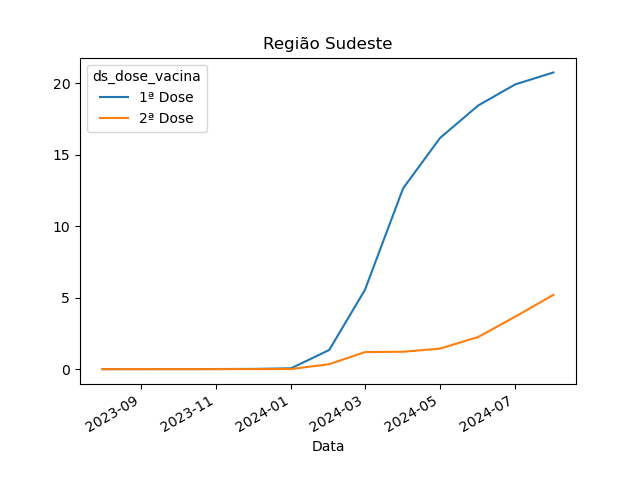
\includegraphics[width=0.85\linewidth]{imagens/Dengue-Sudeste-Cumulativo-mes}
    \caption{Dengue - Cumulativo (últimos 12 meses) por mês - Sudeste}
    \label{fig:dengue-sudeste-cumulativo-mes}
\end{figure}
\begin{figure}[H]
    \centering
    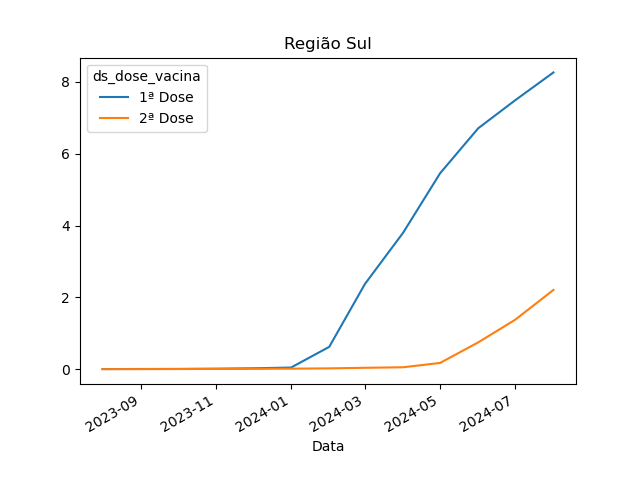
\includegraphics[width=0.85\linewidth]{imagens/Dengue-Sul-Cumulativo-mes}
    \caption{Dengue - Cumulativo (últimos 12 meses) por mês - Sul}
    \label{fig:dengue-sul-cumulativo-mes}
\end{figure}

\subsubsection{HPV4}
\begin{figure}[H]
    \centering
    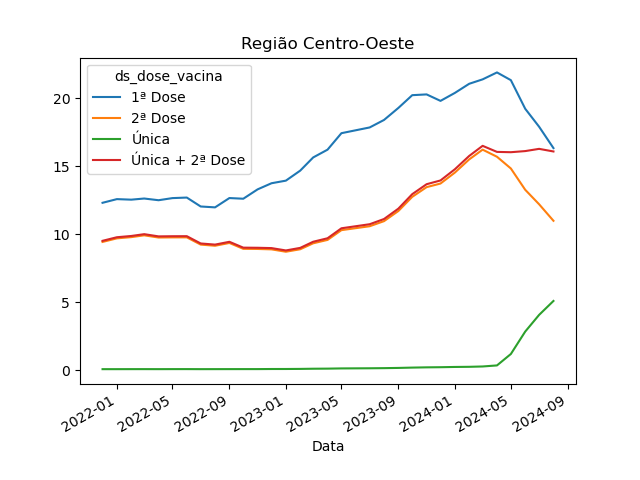
\includegraphics[width=0.85\linewidth]{imagens/HPV4-Centro-Oeste-Cumulativo-mes}
    \caption{HPV4 - Cumulativo (últimos 12 meses) por mês - Centro-Oeste}
    \label{fig:HPV4-centro-oeste-cumulativo}
\end{figure}
\begin{figure}[H]
    \centering
    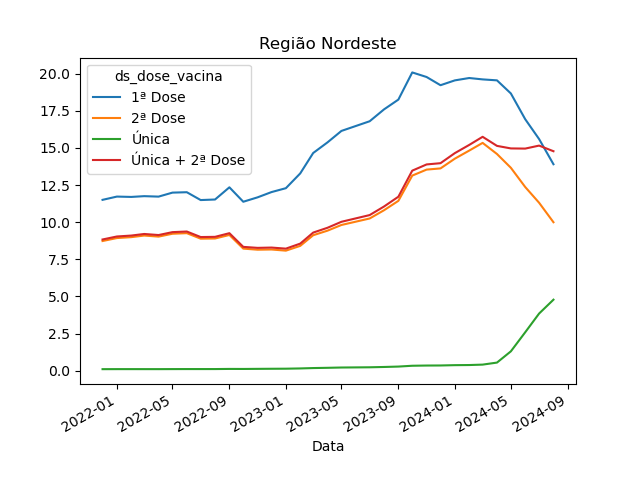
\includegraphics[width=0.85\linewidth]{imagens/HPV4-Nordeste-Cumulativo-mes}
    \caption{HPV4 - Cumulativo (últimos 12 meses) por mês - Nordeste}
    \label{fig:HPV4-nordeste-cumulativo-mes}
\end{figure}
\begin{figure}[H]
    \centering
    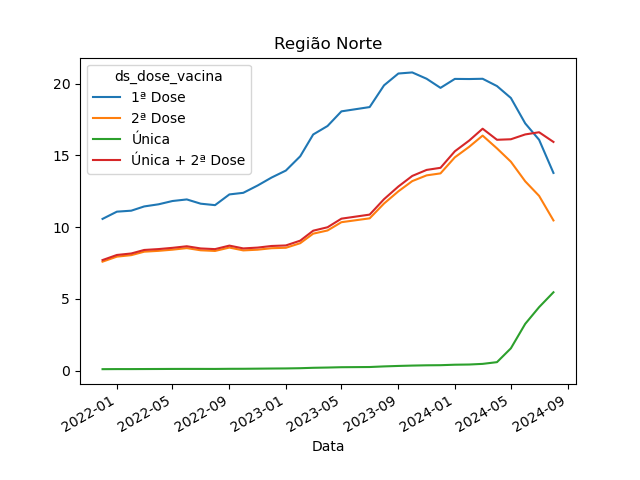
\includegraphics[width=0.85\linewidth]{imagens/HPV4-Norte-Cumulativo-mes}
    \caption{HPV4 - Cumulativo (últimos 12 meses) por mês - Norte}
    \label{fig:HPV4-norte-cumulativo-mes}
\end{figure}
\begin{figure}[H]
    \centering
    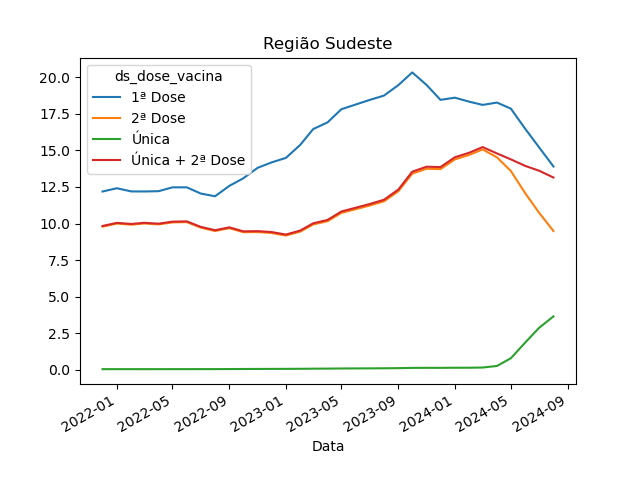
\includegraphics[width=0.85\linewidth]{imagens/HPV4-Sudeste-Cumulativo-mes}
    \caption{HPV4 - Cumulativo (últimos 12 meses) por mês - Sudeste}
    \label{fig:HPV4-sudeste-cumulativo-mes}
\end{figure}
\begin{figure}[H]
    \centering
    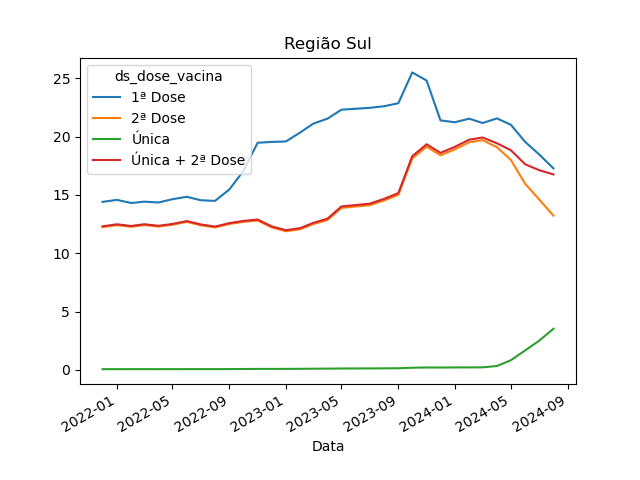
\includegraphics[width=0.85\linewidth]{imagens/HPV4-Sul-Cumulativo-mes}
    \caption{HPV4 - Cumulativo (últimos 12 meses) por mês - Sol}
    \label{fig:HPV4-sul-cumulativo-mes}
\end{figure}

\subsubsection{MenACWY}
\begin{figure}[H]
    \centering
    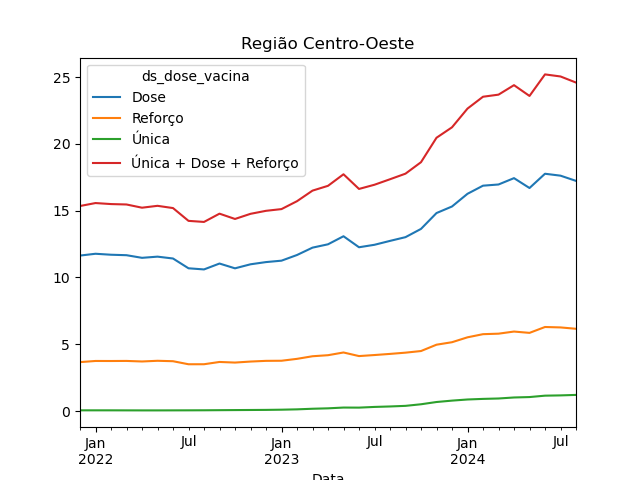
\includegraphics[width=0.85\linewidth]{imagens/MenACWY-Centro-Oeste-Cumulativo-mes}
    \caption{MenACWY - Cumulativo (últimos 12 meses) por mês - Centro-Oeste}
    \label{fig:MenACWY-centro-oeste-cumulativo}
\end{figure}
\begin{figure}[H]
    \centering
    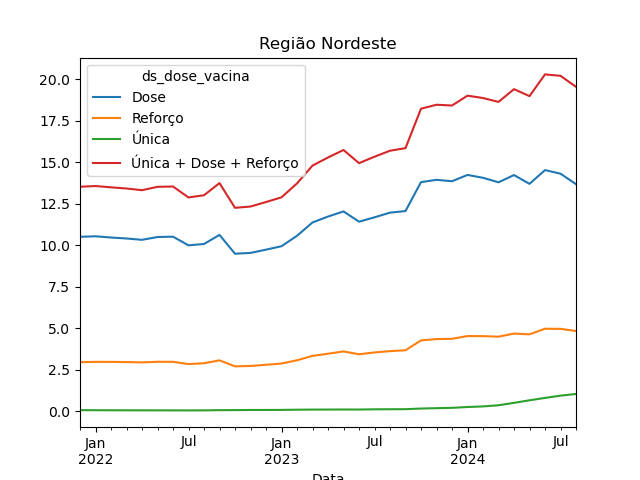
\includegraphics[width=0.85\linewidth]{imagens/MenACWY-Nordeste-Cumulativo-mes}
    \caption{MenACWY - Cumulativo (últimos 12 meses) por mês - Nordeste}
    \label{fig:MenACWY-nordeste-cumulativo-mes}
\end{figure}
\begin{figure}[H]
    \centering
    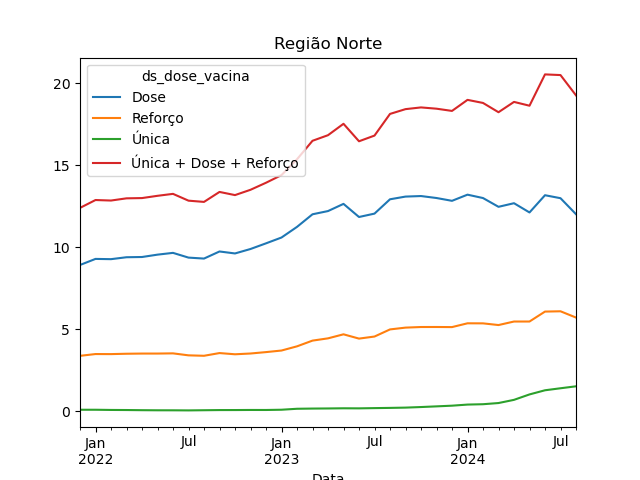
\includegraphics[width=0.85\linewidth]{imagens/MenACWY-Norte-Cumulativo-mes}
    \caption{MenACWY - Cumulativo (últimos 12 meses) por mês - Norte}
    \label{fig:MenACWY-norte-cumulativo-mes}
\end{figure}
\begin{figure}[H]
    \centering
    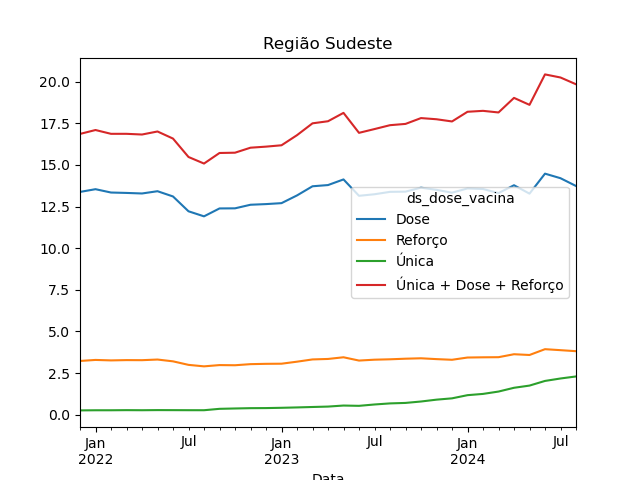
\includegraphics[width=0.85\linewidth]{imagens/MenACWY-Sudeste-Cumulativo-mes}
    \caption{MenACWY - Cumulativo (últimos 12 meses) por mês - Sudeste}
    \label{fig:MenACWY-sudeste-cumulativo-mes}
\end{figure}
\begin{figure}[H]
    \centering
    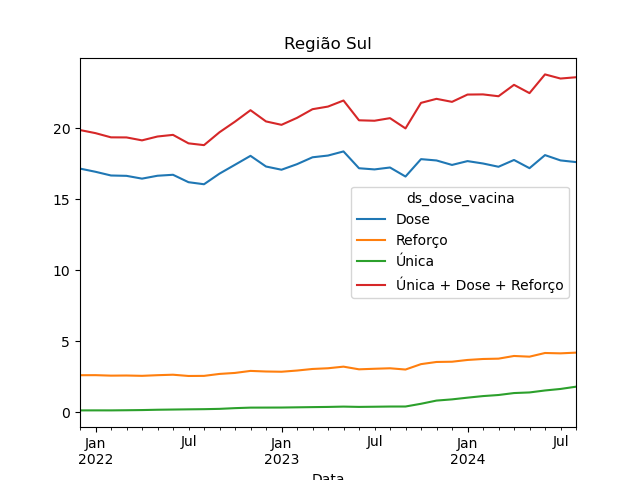
\includegraphics[width=0.85\linewidth]{imagens/MenACWY-Sul-Cumulativo-mes}
    \caption{MenACWY - Cumulativo (últimos 12 meses) por mês - Sol}
    \label{fig:MenACWY-sul-cumulativo-mes}
\end{figure}


\subsection{Análise}
Para todas as vacinas é possível verificar um decréscimo nas taxas de vacinação nos 3 últimos meses dos dados. Um fator é que os dados do RNDS seguem sendo atualizados por diversos motivos: órgãos municipais e estaduais de saúde muitas vezes enviam dados com atraso, especialmente quando a coleta é feita offline; conforme os dados são recebidos pelo DataSUS, eles passam por validações e limpeza antes de serem adicionados ao RNDS; alguns dados precisam ser revistos e os órgãos e unidades responsáveis são acionadas.

É possível verificar que, na vacina contra a dengue, não existem muitas aplicações até fevereiro de 2024. Após esse período, que coincide com a inclusão dessa vacina no Calendário Básico, todas as regiões tiveram um aumento significativo nas aplicações. A região Centro-Oeste, seguida pela região Sudeste, tiveram os aumentos mais significativos em aplicações, enquanto a região Sul teve o menor aumento de todas. Apesar disso, em todas as regiões a cobertura vacinal segue aumentando, com uma cobertura de 25\% no Centro-Oeste, 20\% no Sudeste, 10\% no Norte e Nordeste e 8\% no Sul. Já a cobertura completa mal chega a 5\% no Centro-Oeste e Sudeste e a 2\% no restante. Todos valores muito aquém da meta de 90\%.

A vacina HPV4 segue uma tendência de aumento nas aplicações e vem sendo substituída pela dose única, o que deve auxiliar no aumento dos índices de cobertura vacinal completa. Sua cobertura vacinal segue uma tendência de aumento, com um percentual de quase 20\% em todas as regiões (a região Sul chegou a quase 25\% em outubro de 2023). A cobertura vacinal completa mostra uma tendência de crescimento e está ao redor de 15\% em todas as regiões. Todos muito aquém da meta de 90%.

A vacina MenACWY teve uma tendência de aumento de aplicações em 2023, que reflete na maior cobertura que vemos em 2024. Porém, as taxas de aplicação reduziram em 2024 o que, se não for revertido, vai impactar a cobertura vacinal de 2025. Essa vacina possui 3 tipos de doses nos registros do público alvo: Dose, Reforço e Única. A dose é especificada como "Reforço" quando a criança ou adolescente já recebeu esse imunobiológico previamente na infância. Portanto, todos essas doses são consideradas válidas para a cobertura vacinal. A cobertura vacinal completa está em torno de 24\% nas regiões Centro-Oeste e Sul, e 19\% nas outras 3 regiões. Ainda baixo frente a meta de 80\%.

Existe uma queda abrupta nas doses aplicadas da vacina MenACWY em junho de 2023, porém isso parece estar relacionado a uma falha nos dados do RNDS, pois o período de junho de 2023 possui um volume de dados que é uma ordem de grandeza a menor que todos os outros meses.

\section{Resultados} \label{sec:resultados}
A análise exploratória dos dados permitiu uma avaliação das taxas de aplicação de doses e da cobertura vacinal das vacinas propostas no trabalho. A vacina contra a dengue é mais recente e não possui uma quantidade significativa de dados para permitir uma análise mais profunda. Os dados, disponibilizados desde agosto de 2024, incluem as doses aplicadas desde janeiro de 2021 e se mostram valiosos na análise da fração de adolescentes que receberam as vacinas do Calendário Básico e a cobertura que elas seguem oferecendo a essa população alvo.

A criação de scripts para armazenamento e processamento dos dados e geração de gráficos se mostrou muito valiosa durante a análise, reduziu a capacidade de hardware necessário e permitiu automatizar o processo conforme mais dados foram coletados dos portais de dados abertos. Dentre as ferramentas testadas estiveram: pandas, pyarrow, vaex, dask, Orange, Google Cloud e utilitários de linha de comando Linux.

O tamanho total dos arquivos de doses aplicadas, compactados individualmente por mês no formato \emph{zip}, ficou em 56 GB. Isso impossibilitou utilização de qualquer ferramenta sem processamento \emph{out-of-core}, ou seja, que fosse capaz de fazer uma leitura sob demanda dos dados sem precisar carregar tudo para a \emph{RAM}. Isso eliminou o Orange e, para o tratamento mais intensivo dos dados, o pandas, pois embora ele permita fazer \emph{chunking} dos dados, isso dificulta a aplicação de funções como \emph{group by}. As ferramentas que suportavam operações \emph{out-of-core} como pyarrow, dask e vaex tiveram problemas durante a importação na exportação dos dados (para um formato mais amigável à operações \emph{out-of-core} como parket), com muitos conflitos de tipos e falha nas conversões. O Google Cloud foi capaz de ler alguns arquivos, mas o ecossistema possui uma curva de aprendizado significativa e uma falta de transparência incômoda sobre custos. Por fim, ferramentas de linha de comando Linux, como \emph{grep}, \emph{cut}, \emph{tr}, \emph{head}, \emph{tail} e \emph{paste} foram capazes de fazer o pré-processamento e importação dos dados para o banco de dados sqlite3. Operações de SQL se mostraram eficientes e simples para particionar, agrupar e filtrar os dados.

\section{Considerações Finais} \label{sec:consideracoes finais}
Os resultados demonstram que é relevante e simples automatizar o processamento dos dados para análises de doses aplicadas e cobertura vacinal em uma população alvo. Os órgãos de saúde federais teriam um grande benefícios em incorporar um processo similar aos portais existentes. Aumentar o nível de detalhamento dos dados geográficos, ao nível de estado e, em especial, município, similar ao Observatório das vacinas \cite{observatorio_das_vacinas_mapa_2020}, iria permitir destacar quais locais precisam de maior atenção, assim como evidenciar os melhores, permitindo investigar seus processos e sucessos.

Uma investigação no atraso da incorporação dos registros no sistema RNDS, identificado pela disparidade entre a data da aplicação da dose e a data de entrada no sistema, permitiria um estudo estatístico, análise das características e causas desses atrasos, identificando pontos importantes para otimização do processo. Poderia avaliar os métodos de entrada (online, offline, SI-PNI, PAS) e características das unidades de atendimento (privada, pública, UBS, USF, localização) para identificar correlações significativas com o atraso.

A falta de estudos abrangentes na cobertura vacinal de adolescentes pelo Calendário Básico e a recente disponibilização dos dados de doses aplicadas indica a possibilidade de mais estudos.

\bibliographystyle{sbc}
\bibliography{tdaitx-unisinos-artigo-tec-eng-sw-aplicada}

\appendix
\section{Apêndice: vacinacao2sqlite.sh}
\begin{minted}[linenos=true]{bash}
#!/bin/bash -eu

if [ "x${1-}" == "x" ]; then
echo "Usage: $0 file.zip [file2.zip] ..."
exit 1
fi


filtro_colunas="co_municipio_paciente
no_municipio_paciente
no_pais_paciente
sg_uf_paciente
sg_vacina
dt_vacina
ds_dose_vacina
ds_vacina
nu_idade_paciente"

SQL_DB="vacinacao.sqlite3"


{
    echo 'CREATE TABLE IF NOT EXISTS vacinacao ('
    for nome_coluna in $filtro_colunas; do
    case $nome_coluna in
    co_*) tipo_coluna='NUMERIC';;
    nu_*) tipo_coluna='INTEGER';;
    *) tipo_coluna='STRING';;
    esac;
    echo "\"$nome_coluna\" $tipo_coluna";
    done | paste -sd ','
    echo ");"
} | tee /dev/stderr | sqlite3 vacinacao.sqlite3 ".read '|cat -'"

for f in "$@"; do
echo "Processando arquivo: $f"
colunas_arquivo=$(unzip -p $1 | head -n1 | tr ';' '\n')
colunas_encontradas=$(echo "$colunas_arquivo" | grep -nxFf <(echo "$filtro_colunas"))
colunas_numeradas=$(echo "$colunas_encontradas" | cut -d: -f1 | paste -sd,)
if [[ $(echo "$filtro_colunas" | wc -l) -ne $(echo "$colunas_encontradas" | wc -l) ]]; then
echo "Erro: nem todas as colunas puderam ser extraídas"
echo "Colunas solicitadas:"
echo "$filtro_colunas"
echo "Colunas encontradas:"
echo "$colunas_encontradas"
exit 1
fi
echo "Gravando colunas:"
echo "$colunas_encontradas"
unzip -p "$f" | cut -s -d';' -f "$colunas_numeradas" | iconv -f ISO-8859-1 -t UTF-8 | tail -n+2 | sqlite3 --csv --separator ";" vacinacao.sqlite3 ".import '|cat -' vacinacao"
done

sqlite3 vacinacao.sqlite3 << EOF
.tables
.schema
select count(*) from vacinacao;
delete from vacinacao where no_pais_paciente!="BRASIL";
delete from vacinacao where co_municipio_paciente=999999 or no_municipio_paciente="INVALIDO";
delete from vacinacao where nu_idade_paciente="";
delete from vacinacao where sg_uf_paciente="" or no_municipio_paciente="" or co_municipio_paciente="";
delete from vacinacao where ds_vacina="" OR sg_vacina="";
select count(*) from vacinacao;
EOF
\end{minted}

\section{Apêndice: Dados do Censo 2022}
URL - Censo 2022 de Grande Regiao, idade, sexo e população

\url{https://sidra.ibge.gov.br/tabela/9514#/n2/all/v/allxp/p/all/c2/allxt/c287/6557,6558,6559,6560,6561,6562,6563,6564,6565,6566,6567,6568,6569,6570,6571,6572,6573,6574,6575,6576,6577,6578,6579,6580,6581,6582,6583,6584,6585,6586,6587,6588,6589,6590,6591,6592,6593,6594,6595,6596,6597,6598,6599,6600,6601,6602,6603,6604,6605,6606,6607,6608,6609,6610,6611,6612,6613,6614,6615,6616,6617,6618,6619,6620,6621,6622,6623,6624,6625,6626,6627,6628,6629,6630,6631,6632,6633,6634,6635,6636,6637,6638,6639,6640,6641,6642,6643,6644,6645,6646,6647,6648,6649,6650,6651,6652,6653,6656,6657,6658,6659/c286/113635/l/v+c286+p,,t+c287+c2}

URL - Censo 2022 - UF, idade, sexo e população

\url{https://sidra.ibge.gov.br/tabela/9514#/n3/all/v/allxp/p/all/c2/allxt/c287/6557,6558,6559,6560,6561,6562,6563,6564,6565,6566,6567,6568,6569,6570,6571,6572,6573,6574,6575,6576,6577,6578,6579,6580,6581,6582,6583,6584,6585,6586,6587,6588,6589,6590,6591,6592,6593,6594,6595,6596,6597,6598,6599,6600,6601,6602,6603,6604,6605,6606,6607,6608,6609,6610,6611,6612,6613,6614,6615,6616,6617,6618,6619,6620,6621,6622,6623,6624,6625,6626,6627,6628,6629,6630,6631,6632,6633,6634,6635,6636,6637,6638,6639,6640,6641,6642,6643,6644,6645,6646,6647,6648,6649,6650,6651,6652,6653,6656,6657,6658,6659/c286/113635/l/v+c286+p,,t+c287+c2/cfg/cod,}

URL - Censo 2022 - Município, idade, sexo e população

\url{https://sidra.ibge.gov.br/tabela/9514#/n6/all/v/allxp/p/all/c2/allxt/c287/6557,6558,6559,6560,6561,6562,6563,6564,6565,6566,6567,6568,6569,6570,6571,6572,6573,6574,6575,6576,6577,6578,6579,6580,6581,6582,6583,6584,6585,6586,6587,6588,6589,6590,6591,6592,6593,6594,6595,6596,6597,6598,6599,6600,6601,6602,6603,6604,6605,6606,6607,6608,6609,6610,6611,6612,6613,6614,6615,6616,6617,6618,6619,6620,6621,6622,6623,6624,6625,6626,6627,6628,6629,6630,6631,6632,6633,6634,6635,6636,6637,6638,6639,6640,6641,6642,6643,6644,6645,6646,6647,6648,6649,6650,6651,6652,6653,6656,6657,6658,6659/c286/113635/l/v+c286+p,,t+c287+c2/cfg/cod,}


\section{Apêndice: censo2sqlite.sh}
\begin{minted}[linenos=true]{bash}
#!/bin/bash -xeu

function filtrar_idades() {
    sed -e "s/Menos de 1 ano/0/" -e "s/ anos ou mais//" -e "s/ anos\?//"
}

function filtrar_sexo() {
    sed -e "s/Homens/H/" -e "s/Mulheres/M/"
}

function separar_estado() {
    sed -E 's/ \(([A-Z]{2})\)/\\";\"\1/'
}

function substituir_por_zeros() {
    sed 's/"-"/0/'
}

sqlite3 vacinacao.sqlite3 "DROP TABLE IF EXISTS censo2022regiao;"
sqlite3 vacinacao.sqlite3 "CREATE TABLE censo2022regiao ( \"no_regiao\" STRING, \"nu_idade\" INTEGER, \"co_sexo\" STRING, \"nu_populacao\" INTEGER);"
tail -n+6 arquivos_censo/censo2022-grande-regiao-todas-idades-sexo.csv | head -n1010 | sed 's/\r//' | filtrar_idades | filtrar_sexo | sqlite3 --csv --separator ";" vacinacao.sqlite3 ".import '|cat -' censo2022regiao"

sqlite3 vacinacao.sqlite3 "DROP TABLE IF EXISTS censo2022uf;"
sqlite3 vacinacao.sqlite3 "CREATE TABLE censo2022uf ( \"co_uf\" INTEGER, \"no_uf\" STRING, \"nu_idade\" INTEGER, \"co_sexo\" STRING, \"nu_populacao\" INTEGER);"
tail -n+6 arquivos_censo/censo2022-uf-todas-idades-sexo.csv | head -n5454 | sed 's/\r//' | filtrar_idades | filtrar_sexo | sqlite3 --csv --separator ";" vacinacao.sqlite3 ".import '|cat -' censo2022uf"

sqlite3 vacinacao.sqlite3 "DROP TABLE IF EXISTS censo2022municipio;"
sqlite3 vacinacao.sqlite3 "CREATE TABLE censo2022municipio ( \"co_municipio\" INTEGER, \"no_municipio\" STRING, \"sg_uf\" STRING, \"nu_idade\" INTEGER, \"co_sexo\" STRING, \"nu_populacao\" INTEGER);"
tail -n+6 arquivos_censo/censo2022-municipio-todas-idades-sexo.csv | head -n1125140 | sed 's/\r//' | filtrar_idades | filtrar_sexo | separar_estado | substituir_por_zeros | sqlite3 --csv --separator ";" vacinacao.sqlite3 ".import '|cat -' censo2022municipio"


### VIEWS
# população do censo por regiao/idade
sqlite3 vacinacao.sqlite3 "CREATE VIEW IF NOT EXISTS censo2022regiao_idade (no_regiao, nu_idade, nu_populacao) as SELECT no_regiao, nu_idade, sum(nu_populacao) as nu_populacao FROM censo2022regiao GROUP BY no_regiao, nu_idade;"

# população do censo por uf/idade
sqlite3 vacinacao.sqlite3 "CREATE VIEW IF NOT EXISTS censo2022uf_idade (sg_uf, nu_idade, nu_populacao) as SELECT sg_uf, nu_idade, sum(nu_populacao) as nu_populacao FROM censo2022uf c, regiao_uf r WHERE r.no_uf=c.no_uf GROUP BY sg_uf, nu_idade;"

# Dengue: doses aplicadas por ano/regiao/tipo dose/idade
sqlite3 vacinacao.sqlite3 "CREATE VIEW IF NOT EXISTS dengue_ano_regiao_dose_idade (nu_ano, no_regiao, sg_vacina, ds_dose_vacina, nu_idade_paciente, nu_doses_aplicadas) as SELECT printf no_regiao, \"Dengue\", ds_dose_vacina, nu_idade_paciente, count(*) as doses_aplicadas FROM vacinacao, regiao_uf WHERE sg_uf=sg_uf_paciente AND nu_idade_paciente>=10 AND nu_idade_paciente<=14 AND (sg_vacina='Dengue' OR sg_vacina='DNG') AND (ds_dose_vacina='1ª Dose' OR ds_dose_vacina='2ª Dose') GROUP BY no_regiao, ds_dose_vacina, nu_idade_paciente;"

# doses 2024 MenACWY por regiao/tipo dose/idade
sqlite3 vacinacao.sqlite3 "CREATE VIEW IF NOT EXISTS vacinacaodoses_menacwy_regiao_dose_idade (no_regiao, sg_vacina, ds_dose_vacina, nu_idade_paciente, nu_doses_aplicadas) as SELECT no_regiao, sg_vacina, ds_dose_vacina, nu_idade_paciente, count(*) as doses_aplicadas FROM vacinacao, regiao_uf WHERE sg_uf=sg_uf_paciente AND nu_idade_paciente>=11 AND nu_idade_paciente<=14 AND (sg_vacina='MenACWY') AND (ds_dose_vacina='Dose' OR ds_dose_vacina='Reforço' OR ds_dose_vacina='Única') GROUP BY no_regiao, ds_dose_vacina, nu_idade_paciente;"

# doses 2024 HPV4 por regiao/tipo dose/idade
sqlite3 vacinacao.sqlite3 "CREATE VIEW IF NOT EXISTS vacinacaodoses_hpv4_regiao_dose_idade (no_regiao, sg_vacina, ds_dose_vacina, nu_idade_paciente, nu_doses_aplicadas) as SELECT no_regiao, sg_vacina, ds_dose_vacina, nu_idade_paciente, count(*) as doses_aplicadas FROM vacinacao, regiao_uf WHERE sg_uf=sg_uf_paciente AND nu_idade_paciente>=9 AND nu_idade_paciente<=14 AND (sg_vacina='HPV4') AND (ds_dose_vacina='1ª Dose' OR ds_dose_vacina='2ª Dose' OR ds_dose_vacina='Única') GROUP BY no_regiao, ds_dose_vacina, nu_idade_paciente;"


# MenACWY: doses anuais por uf/tipo dose/idade
sqlite3 vacinacao.sqlite3 \
"CREATE VIEW IF NOT EXISTS
menacwy_uf_dose_idade (sg_uf, nu_ano, sg_vacina, ds_dose_vacina, nu_idade_paciente, nu_doses_aplicadas) AS
SELECT sg_uf_paciente, nu_ano, sg_vacina, ds_dose_vacina, nu_idade_paciente, nu_doses_aplicadas
FROM vacinacao
WHERE nu_idade_paciente>=11 AND nu_idade_paciente<=14
AND sg_vacina='MenACWY'
AND (ds_dose_vacina='Dose' OR ds_dose_vacina='Reforço' OR ds_dose_vacina='Única')
GROUP BY sg_uf_paciente, nu_ano,ds_dose_vacina, nu_idade_paciente;"

# Dengue: doses mensais por regiao/tipo de dose/idade
sqlite3 vacinacao.sqlite3 \
"CREATE VIEW IF NOT EXISTS
dengue_ano_mes_regiao_dose_idade (no_regiao, nu_ano, nu_mes, sg_vacina, ds_dose_vacina, nu_idade_paciente, nu_doses_aplicadas) AS
SELECT no_regiao, strftime('%Y', dt_vacina) as nu_ano, strftime('%m', dt_vacina) as nu_mes, \"Dengue\",
ds_dose_vacina, nu_idade_paciente, count(*) as doses_aplicadas
FROM vacinacao, regiao_uf
WHERE sg_uf=sg_uf_paciente
AND nu_idade_paciente>=10
AND nu_idade_paciente<=14
AND (sg_vacina='Dengue' OR sg_vacina='DNG') \
AND (ds_dose_vacina='1ª Dose' OR ds_dose_vacina='2ª Dose')
GROUP BY no_regiao, nu_ano, nu_mes, ds_dose_vacina, nu_idade_paciente;"

# MenACWY: doses mensais por regiao/tipo de dose/idade
sqlite3 vacinacao.sqlite3 \
"CREATE VIEW IF NOT EXISTS
menacwy_ano_mes_regiao_dose_idade (no_regiao, nu_ano, nu_mes, sg_vacina, ds_dose_vacina, nu_idade_paciente, nu_doses_aplicadas) AS
SELECT no_regiao, strftime('%Y', dt_vacina) as nu_ano, strftime('%m', dt_vacina) as nu_mes, sg_vacina,
ds_dose_vacina, nu_idade_paciente, count(*) as doses_aplicadas
FROM vacinacao, regiao_uf
WHERE sg_uf=sg_uf_paciente
AND nu_idade_paciente>=11
AND nu_idade_paciente<=14
AND sg_vacina='MenACWY'
AND (ds_dose_vacina='Dose' OR ds_dose_vacina='Reforço' OR ds_dose_vacina='Única')
GROUP BY no_regiao, nu_ano, nu_mes, ds_dose_vacina, nu_idade_paciente;"

# HPV4: doses mensais por regiao/tipo de dose/idade
sqlite3 vacinacao.sqlite3 \
"CREATE VIEW IF NOT EXISTS
hpv4_ano_mes_regiao_dose_idade (no_regiao, nu_ano, nu_mes, sg_vacina, ds_dose_vacina, nu_idade_paciente, nu_doses_aplicadas) AS
SELECT no_regiao, strftime('%Y', dt_vacina) as nu_ano, strftime('%m', dt_vacina) as nu_mes, sg_vacina,
ds_dose_vacina, nu_idade_paciente, count(*) as doses_aplicadas
FROM vacinacao, regiao_uf
WHERE sg_uf=sg_uf_paciente
AND nu_idade_paciente>=9
AND nu_idade_paciente<=14
AND sg_vacina='HPV4'
AND (ds_dose_vacina='1ª Dose' OR ds_dose_vacina='2ª Dose' OR ds_dose_vacina='Única')
GROUP BY no_regiao, nu_ano, nu_mes, ds_dose_vacina, nu_idade_paciente;"

# cobertura vacinal mensal de adolescentes por regiao/tipo de dose/faixa-etaria
sqlite3 vacinacao.sqlite3 \
"CREATE VIEW IF NOT EXISTS
cobertura_regiao_adolescentes_ano_mes (nu_ano, nu_mes, sg_vacina, ds_dose_vacina, ds_faixa_etaria,
no_regiao, nu_doses_aplicadas, nu_populacao, nu_cobertura_vacinal) AS
SELECT nu_ano, nu_mes, sg_vacina, ds_dose_vacina, format('%u-%u',min(nu_idade_paciente),max(nu_idade_paciente)),
v.no_regiao, sum(nu_doses_aplicadas) as nu_doses_aplicadas, sum(nu_populacao),
(100.0 * sum(nu_doses_aplicadas) / sum(nu_populacao))
FROM censo2022regiao_idade c, dengue_ano_mes_regiao_dose_idade v
WHERE c.no_regiao=v.no_regiao
AND v.nu_idade_paciente=(c.nu_idade+nu_ano-2022)
GROUP BY nu_ano, nu_mes, c.no_regiao, v.ds_dose_vacina
UNION
SELECT nu_ano, nu_mes, sg_vacina, ds_dose_vacina, format('%u-%u',min(nu_idade_paciente),max(nu_idade_paciente)),
v.no_regiao, sum(nu_doses_aplicadas) as nu_doses_aplicadas, sum(nu_populacao),
(100.0 * sum(nu_doses_aplicadas) / sum(nu_populacao))
FROM censo2022regiao_idade c, menacwy_ano_mes_regiao_dose_idade v
WHERE c.no_regiao=v.no_regiao
AND v.nu_idade_paciente=(c.nu_idade+nu_ano-2022)
GROUP BY nu_ano, nu_mes, c.no_regiao, v.ds_dose_vacina
UNION
SELECT nu_ano, nu_mes, sg_vacina, ds_dose_vacina, format('%u-%u',min(nu_idade_paciente),max(nu_idade_paciente)),
v.no_regiao, sum(nu_doses_aplicadas) as nu_doses_aplicadas, sum(nu_populacao),
(100.0 * sum(nu_doses_aplicadas) / sum(nu_populacao))
FROM censo2022regiao_idade c, hpv4_ano_mes_regiao_dose_idade v
WHERE c.no_regiao=v.no_regiao
AND v.nu_idade_paciente=(c.nu_idade+nu_ano-2022)
GROUP BY nu_ano, nu_mes, c.no_regiao, v.ds_dose_vacina
ORDER BY nu_ano, sg_vacina, v.no_regiao, nu_mes, nu_doses_aplicadas DESC;"


# Tabela Regioes/UF
sqlite3 vacinacao.sqlite3 "DROP TABLE IF EXISTS regiao_uf;"
sqlite3 vacinacao.sqlite3 "CREATE TABLE regiao_uf ( \"no_regiao\" STRING, \"sg_uf\" STRING, \"no_uf\" STRING, \"co_uf\" INTEGER);"
echo "Centro-Oeste,DF,Distrito Federal,53
Centro-Oeste,GO,Goiás,52
Centro-Oeste,MS,Mato Grosso do Sul,50
Centro-Oeste,MT,Mato Grosso,51
Nordeste,AL,Alagoas,27
Nordeste,BA,Bahia,29
Nordeste,CE,Ceará,23
Nordeste,MA,Maranhão,21
Nordeste,PB,Paraíba,25
Nordeste,PE,Pernambuco,26
Nordeste,PI,Piauí,22
Nordeste,RN,Rio Grande do Norte,24
Nordeste,SE,Sergipe,28
Norte,AC,Acre,12
Norte,AP,Amapá,16
Norte,AM,Amazonas,13
Norte,PA,Pará,15
Norte,RO,Rondônia,11
Norte,RR,Rorraima,14
Norte,TO,Tocantins,17
Sudeste,ES,Espírito Santo,32
Sudeste,MG,Minas Gerais,31
Sudeste,RJ,Rio de Janeiro,33
Sudeste,SP,São Paulo,35
Sul,PR,Paraná,41
Sul,RS,Rio Grande do Sul,43
Sul,SC,Santa Catarina,42" | sqlite3 --csv vacinacao.sqlite3 ".import '|cat -' regiao_uf"
\end{minted}

\section{Apêndice: geradorDeGraficos.py}

\begin{minted}[linenos=true]{python}
    import sqlite3
    import pandas as pd
    import matplotlib.pyplot as plt
    conn = sqlite3.connect("vacinacao.sqlite3")

    sql = """select * from cobertura_regiao_adolescentes_ano_mes"""

    data = pd.read_sql(sql, conn)
    #data
    # criar campo de data para facilitar manipulacao tempora dos dados
    data['Data'] = pd.to_datetime(data['nu_ano'] + "-" + data['nu_mes'])

    # remover registros de setembro, que ainda não abrangem o mês inteiro
    data.drop(data[data['Data'] >= pd.Timestamp(2024,9,1)].index, inplace=True)
    doses_aplicadas = data.pivot_table(
    index=["sg_vacina", "no_regiao", "ds_dose_vacina"],
    columns=["Data"],
    values="nu_cobertura_vacinal",
    aggfunc="sum"
    )
    #doses_aplicadas
    da_reg = doses_aplicadas.loc['Dengue'].dropna(axis=1)
    #cv_reg['Completo'] = cv['reg

    for reg in da_reg.index.levels[0]:
    da_dose = da_reg.loc[reg].T
    ax = da_dose.plot()
    ax.set_title("Região " + reg)
    ax.figure.savefig('imagens/Dengue-' + reg + '-Aplicacoes-mes.png')

    ax = da_dose.expanding().sum().dropna().plot()
    ax.set_title("Região " + reg)
    ax.figure.savefig(imagens/Dengue-' + reg + '-Cumulativo-mes.png')
    #cv.index.levels[0]
    #cv.index.unique("sg_vacina")
    for vac in ['HPV4', 'MenACWY']:
    da_reg = doses_aplicadas.loc[vac].dropna(axis=1)
    for reg in da_reg.index.levels[0]:
    da_dose = da_reg.loc[reg].T
    if vac == 'HPV4':
    da_dose['Única + 2ª Dose'] = da_dose['Única'] + da_dose['2ª Dose']
    else:
    da_dose['Única + Dose + Reforço'] = da_dose['Única'] + da_dose['Dose'] + da_dose['Reforço']
    ax = da_dose.plot()
    ax.set_title("Região " + reg)
    ax.figure.savefig('artigo-tecnico/unisinos-paper-eng-sw-aplicada/imagens/' + vac + '-' + reg + '-Aplicacoes-mes.png')

    ax = da_dose.rolling(window=12, closed='right').sum().dropna().plot()
    ax.set_title("Região " + reg)
    ax.figure.savefig('artigo-tecnico/unisinos-paper-eng-sw-aplicada/imagens/' + vac + '-' + reg + '-Cumulativo-mes.png')
\end{minted}
\end{document}
